
\label{sect:template_training}

In this section, we will present an approach for learning SED templates directly from broadband photometry, using a modified version of the algorithm developed in \citet{Budavari2000b}. 
If we assume that the galaxies in our data set are sampled from a small set of underlying spectra, the SED templates, and we know the spectroscopic redshift for each galaxy, we can shift the photometry to the restframe and treat each observation of a redshifted galaxy as a \textit{restframe observation} of one of the templates with a different set of effective filters. 
With a large enough data set, the wavelengths of the effective filters will overlap substantially. 
This over-sampling allows us to recover higher resolution features in the templates, even though the data are low resolution observations of different galaxies.

Let us assume we have a set of SED templates as a starting point, which can represent rudimentary guesses and need not resemble true galaxy spectra. 
In the first part of this section, we describe a method by which we create a training set of broadband photometry for each template from a large data set of galaxy photometry. 
In the second part, we derive the perturbation algorithm that is used to train each SED template on its corresponding photometry set. 
The full training algorithm is an expectation maximization that consists of iterating these two steps: matching photometry to templates, and perturbing templates to better match the photometry.
This process is iterated until the SED templates converge. 
In the final part, we discuss a heuristic for selecting the training hyperparameters.




\subsection{Matching Photometry Sets}
\label{sect:training_sets}
        
Assume we have a set of naive SED templates and a large set of observed fluxes, $\{f_m\}$, with known spectroscopic redshifts, $z_m$. 
Our goal is to train each template on an appropriate subset of the $\{f_m\}$, so that the naive templates better represent the colors of the galaxies. 
To assemble these training sets, we consider subsets $\{f_n\} \subset \{f_m\}$, corresponding to the observed fluxes of a single galaxy at redshift $z$, where the subscript $n$ denotes different filters. 
We compare these observed fluxes with the template fluxes $\{\hat{f}_n\}$, where
\begin{align}
    \hat{f}_n &= \int S\left(\frac{\lambda}{1+z}\right) R^n(\lambda) d\lambda, \label{eq:calc_flux1}
\end{align}
$S(\lambda)$ is an SED template, and $R^n(\lambda)$ is the normalized response function of the filter used to measure the flux $f_n$.
For photon counting detectors,
\begin{align}
    R(\lambda) = \frac{\lambda \, T(\lambda)}{\int \lambda \, T(\lambda) d\lambda},
\end{align}
where $T(\lambda)$ is the system response function that captures the transmittance of the atmosphere and the response of the detector \citep{Bessell2005}.

The observed fluxes are assigned to the template whose colors are most similar, which is determined by normalizing the observed and template fluxes in the same band and picking the template that minimizes the squared differences of the fluxes. 
The normalization band is chosen by selecting the band for which the ratio $\hat{f}_n / f_n$ is the median of the flux ratios for that galaxy. 
By performing this matching and renormalization for each galaxy in the photometry set, we associate a subset of the galaxies (and the corresponding photometry) to each template.

Examining how the galaxies are assigned to the individual templates is helpful in selecting the initial set of templates.
The initial templates should be chosen so that the matching algorithm roughly divides the galaxies by their colors.
It is also important that each set contains a sufficient number of fluxes distributed across the wavelengths of interest, as the perturbation algorithm derived in the next section relies on over-sampling to reconstruct higher resolution features of the SED templates.



\subsection{The Perturbation Algorithm}
\label{sect:perturbation}

Assume we have a set of photometry, $\{f_n\}$, which constitute observations of the same underlying SED template, $S(\lambda)$, at various known redshifts, $z_n$. 
These observed fluxes should approximately match the template fluxes calculated via Equation \ref{eq:calc_flux1}. 
However, we can also calculate the template fluxes by imagining that we are observing the template in its rest frame using a set of effective, blueshifted filters:
\begin{align}
    \hat{f}_n = \int S(\lambda) \, R^n[(1+z_n)\lambda] \, d[(1+z_n)\lambda]. \label{eq:calc_flux2}
\end{align}

We wish to perturb the template so that the template fluxes, $\hat{f}_n$, better match the observed fluxes, $f_n$. 
Replacing $S(\lambda)$ with the discrete representation $s_k$, where k indexes wavelength bins, we can define the cost function (\citealt{Budavari2000b} Equation 7):
\begin{align}
    \chi^2 =
    \sum_n \frac{1}{\sigma_n^2}(\hat{f}_n(\{\hat{s}_k\}) - f_n)^2 + 
    \sum_k \frac{1}{\Delta_k^2}(\hat{s}_k - s_k)^2, \label{eq:cost_function}
\end{align}
where $\hat{s}_k$ is a new template derived by perturbing $s_k$.
The optimum perturbation to $s_k$ can then be found via a multidimensional minimization of the cost function. 
The first term in Equation \ref{eq:cost_function} penalizes differences between the observed fluxes and the perturbed template fluxes, weighted according to $\sigma_n$ (the fractional error of the measured flux). 
The perturbed template fluxes can be calculated with a discretized version of Equation \ref{eq:calc_flux2}:
\begin{align}
    \hat{f}_n(\{\hat{s}_k\}) = \sum_k \hat{s}_k \, r_{k'}^n \Delta\lambda_{k'}
\end{align}
where $r_k^n$ is the discrete representation of $R^n(\lambda)$, $k'$ is the wavelength bin corresponding to $\lambda_{k'} = (1+z_n) \lambda_k$ and $\Delta\lambda_{k'} = (1+z_n)\Delta\lambda_k$, where $\Delta\lambda_k$ is the width of wavelength bin k. 
The second term in Equation \ref{eq:cost_function} penalizes large perturbations, weighted by the hyperparameters $\Delta_k$. 
This parameter controls learning rate and also helps stabilize the results. 
See the next section for more details. 

We follow \citet{Budavari2000b} by introducing the simplifying perturbation and constant terms: 
\begin{align}
    \begin{gathered}
        \xi_k = \hat{s}_k - s_k \\
        g_n = f_n - \sum_k s_k \, r_{k'}^n \Delta\lambda_{k'}.
    \end{gathered}
\end{align} 
Then, we have:
\begin{align}
    \chi^2 = 
    \sum_n \frac{1}{\sigma_n^2} \left( g_n - \sum_k \xi_k \,  r_{k'}^n \Delta\lambda_{k'} \right)^2 +
    \sum_k \frac{\xi_k^2}{\Delta_k^2},
\end{align}
which can be analytically minimized:
\begin{align}
    \frac{\partial \chi^2}{\partial \xi_l} = 0 \implies \sum_k M_{lk} \xi_k = \nu_l.
\end{align}
The matrix $M$ and vector $\nu$ are defined
\begin{align}
    \begin{gathered}
        M_{lk} = \sum_n \frac{1}{\sigma_n^2} (r_{l'}^n \Delta\lambda_{l'}) (r_{k'}^n \Delta\lambda_{k'}) + \frac{\delta_{lk}}{\Delta_k^2}, \\
        \nu_l = \sum_n \frac{g_n}{\sigma_n^2} (r_{l'}^n \Delta\lambda_{l'}),
    \end{gathered}
\end{align}
where $\delta_{lk}$ is the Kronecker delta.
One can numerically solve for $\xi$. 
The perturbed spectrum is then $\hat{s}_k = s_k + \xi_k$. 

\begin{figure}
    \centering
    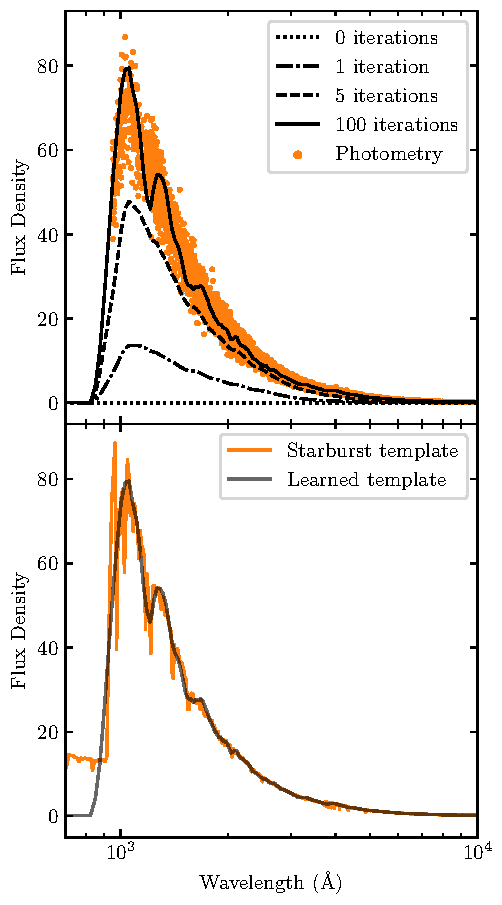
\includegraphics{figures/training_example.pdf}
    \caption{Perturbing a naive template, in this case a flat line, to better match a photometry set. Top: the orange points are simulated observations of the 5Myr starburst template from \citet{Coe2006a} at 1,000 random redshifts in the range z=0 to z=3 using the $ugrizY$ filters listed in Table \ref{tab:filters}. The simulated photometry has 10\% Gaussian error. The template is shown after various stages of the training. Bottom: the learned template is plotted with the original starburst template.}
    \label{fig:pert_ex}
\end{figure}

Iterating the perturbation changes the shape of the template SED to better match the measured photometry, as shown in \citet{Budavari2000b}. 
An example of this process can be seen in Figure \ref{fig:pert_ex}. 
Fluxes in the $ugrizY$ filters listed in Table \ref{tab:filters} were calculated for a starburst galaxy template at 1000 random redshifts $z < 3$. 
Starting with an $S(\lambda) = 0$ template SED, the perturbation algorithm is applied iteratively. 
After 100 iterations, the trained template closely matches the original template in the wavelength range for which photometry exists. 
While the trained template is a smoothed version of the original, high resolution features have been recovered, despite the relatively low resolution of the filters. 
In practice, higher $\Delta_k$ can be chosen so that fewer iterations are required in the training; a lower value was chosen here so that the effects of successive iterations can be more clearly seen.
See Section \ref{sect:hyperparameters} for further discussion of selecting the hyperparameters.

The perturbation algorithm changes the shape of the template SED's so that re-running the photometry matching will now result in different subsets of galaxies assigned to each template.
The full training algorithm is iterated until the SED templates converge.




\subsection{Selecting Hyperparameters}
\label{sect:hyperparameters}

The success of the training algorithm depends on the chosen hyperparameters.
The first is the number of templates. 
As discussed in Section \ref{sect:training_sets}, this choice can be made by using the photometry matching algorithm and choosing the appropriate number of templates to approximately separate out the different spectral shapes displayed in the photometry.
For further discussion of how the number of templates affects photo-z results, see Section \ref{sect:photoz_results}.

The rest of the hyperparameters consist of the set of $\Delta_k$.
These parameters, which set the relative weighting of the regularization term in Equation \ref{eq:cost_function}, determine the stability and speed of the training algorithm.
If the $\Delta_k$ are too large, training will be very slow and a large number of iterations will be required. 
If the $\Delta_k$ are too low, the training becomes unstable and the final templates will be over-fit.
Here we present a heuristic for selecting an appropriate value to balance these two extremes.

For the work presented below, the index $k$ is dropped, so that $\Delta \equiv \Delta_k$ has a single value for each training set that is independent of wavelength. 
In choosing the appropriate value of $\Delta$ for each training set, it is desirable to select a value that corresponds to a constant ratio, $w$, of the flux and regularization terms in Equation \ref{eq:cost_function}. 
The necessary value of $\Delta$ will vary by training set, as the number of terms in the sum over fluxes (i.e. the sum over $n$ in Equation \ref{eq:cost_function}) will vary by training set. 
To this end, we make the following approximation:
\begin{align}
    \frac{\sum_k \left(\hat{s}_k - s_k \right)^2}{\sum_n \left(\hat{f}_n - f_n \right)^2} \sim \frac{N_k}{N_n},
\end{align}
where $N_k \equiv \sum_k$ and $N_n \equiv \sum_n$. 
This permits the following approximation of the ratio $w$: 
\begin{align}
    w = \frac{\sum_k \frac{1}{\Delta^2} \left(\hat{s}_k - s_k \right)^2}{\sum_n \frac{1}{\sigma_n^2} \left(\hat{f}_n - f_n \right)^2} \sim \frac{N_k/\Delta^2}{N_n/\Bar{\sigma}^2},
\end{align}
where $\Bar{\sigma} = \sum_n \sigma_n/N_n$. 
Then, for a desired ratio $w$, the requisite $\Delta$ can be approximated:
\begin{align}
    \Delta \simeq \Bar{\sigma} \sqrt{\frac{N_k}{w N_n}}.
\end{align}
In practice, we have found that $w = \mathcal{O}(1)$ works well.
The results of the training are relatively robust to the selection of $w$, in that changing $w$ by, for example, a factor of 2 yields similar results.